\documentclass[a4paper,12pt,openany]{report}

\usepackage{titling}
\usepackage[margin=0.5in,headsep=0.25in,footskip=0.25in]{geometry}
\usepackage{graphicx}
\usepackage{float}


\newcommand{\subtitle}[1]{
	\posttitle{
		\par\end{center}
		\begin{center}\large#1\end{center}
		\vskip0.5em
	}
}

\setlength{\parindent}{12pt}


% document
\begin{document}

% Title Page
\title{CITS3001 Algorithms and Artificial Intelligence}
\subtitle{Threes Artificial Intelligence Project}
\author{Mitchell Pomery (21130887)\\
Kieran Hannigan (21151118)}
\maketitle
\clearpage

% Introduction
\section*{Introduction}

% What is Threes
\paragraph \indent
We were tasked with the creation of an artificial intelligence to play the game Threes\cite{threes}, aiming to get the highest score possible given a board and a list of upcoming tiles.
Threes is a simple mobile game where you are given a four by four grid occupied by tiles.
The aim is to merge tiles until the board is full and no more merges are possible, or until there are no tiles left to be added to the board.
Each move (left, right, up or down) moves each tile one space on the grid if it is free, or merges it with the tile it moves into if conditions are met.
You are only able to merge a one tile with a two tile, and any other tile with one of the same number.

\begin{figure}[h!]
	\caption{An Example Threes Board}
	\centering 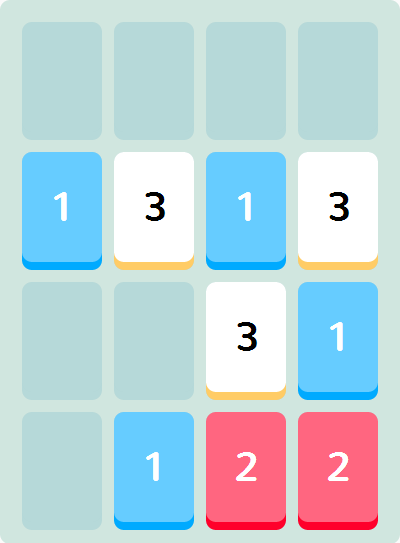
\includegraphics[scale=0.25]{images/examplethreesboard}
\end{figure}

% What Exactly Are We doing


% Specs
\paragraph \indent
The specifications for the threes bot stated three main requirements that were considered during the design and implimentation of the algorithms.
Due to the fact that all upcoming tiles are known, the artificial intelligence is able to look infinitely into the future.
Tile placement is not random, meaning that each move will only have one known outcome and so moving and placing the next tile can be seen as one action.
A full search of every possible combination of moves is not possible, as the bot is required to make five to ten moves per second.

% Language Choice
\paragraph \indent
Python was chosen as an initial language for the artificial intelligence due to the ability to rapidly prototype different algorithms.
The intention was to later port the final algorithm to C to see an increase in performance, and henceforth let the bot look further into the future for better moves.
Unfortunately we ran out of time to impliment the artificial intelligence in C, but did program the basics for Threes.

% Algorithms
\section*{Algorithms}

\subsection*{Making Moves}
\paragraph \indent
There are two ways the moves can be implimented in the bot, either each possible move seperately, or by rotating the board and treating all moves as the one direction.
We implimented the latter of the two algorithms, as it allows us to reduce the amount of code written.
However rotating a sixteen by sixteen board can take several operations, so to avoid this, instead of rotating the board, we rotate the co-ordinates.

\subsection*{Naive}
\paragraph \indent
Initially an naive algorithm was implimented to play Threes one move at a time.
It would look at the four possible moves, left, right, up and down, and take the one that gives it the highest score.
The naive algorithm is useful as a heuristic later in the A* implimentation.

\subsection*{Minimax}
\paragraph \indent
A minimax implimentation was investigated due to the similarities between Threes and 2048, and the already existing 2048 AI by Matt Overlan\cite{2048ai}.
In 2048 the next tile is places randomly, while the specifications state that the next tile will be placed in the lexographically lowest location.
This difference means that the Threes bot does not end up playing against anything, and so minimax is not a relevant algorithm.

\subsection*{A Star}
\paragraph \indent
A* by definition finds the least-cost path from the initial state to a goal state.
The goal state in a game of Threes is the highest scoring full board, meaning that the algorithm needs to avoid filling the board for as long as possible.

% bibliography
\begin{thebibliography}{20} 
 \bibitem{threes} THREES - A tiny puzzle that grows on you. 2014. THREES - A tiny puzzle that grows on you. [ONLINE] Available at: http://asherv.com/threes/. [Accessed 28 May 2014].
 \bibitem{2048ai} 2048. 2014. 2048. [ONLINE] Available at: http://ov3y.github.io/2048-AI/. [Accessed 28 May 2014].
\end{thebibliography} 


\end{document}